\chapter{Results}

\section{The article}

\subsection{Scan Coverage}

The goal of the UAVs is to scan the full map once per hour. In theory, with a speed of 150 km/h, the maximum scan speed is 0.083 km\textsuperscript{2}/second/UAV. So with an area of 900 km\textsuperscript{2}, the fastest time to cover the full area is 18 minutes. The figure \ref{randomcoverage} and the figure \ref{pheromonecoverage} represent the coverage data from the mobility models.

\begin{figure}[h]
\caption{\label{randomcoverage} Random mobility coverage}
   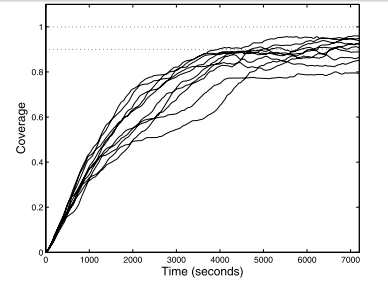
\includegraphics{../images/random_coverage.png}
\end{figure}

\newpage

\begin{figure}[!h]
\caption{\label{pheromonecoverage} Pheromone mobility coverage}
   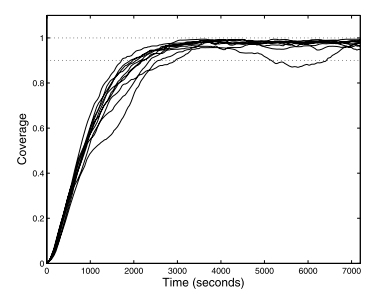
\includegraphics{../images/pheromone_coverage.png}
\end{figure}

For the random model, we see that it need more than 83 minutes to reach 80 percents of coverage. Whereas the pheromone model reach the 90 percents in 60 minutes. Comparing the two models, the pheromone model has a much higher coverage rate.

\newpage

\subsection{Scan Characteristic}

In Figure \ref{randomchar} and Figure \ref{pheromonechar}, the solid lines represent the probability distribution of each models. This curve permits to calculate the probability of the next scan.\\
To know the probability of the next scan between the time t1 and t2, we have to calculate the area under the curve between t1 and t2.\\
So to meet with the requirement of one scan of the map per hour, the curve must be 0 at 1 hour. However none models reach 0 before one hour, because no model manages to achieve full coverage, the pheromone model manages well to avoid rescanning a recently scanned area. We can see that on the graphic : the median curve follows the dashed line at time between 0 seconds and 1000 seconds.

\begin{figure}[!h]
\caption{\label{randomchar} Random mobility}
   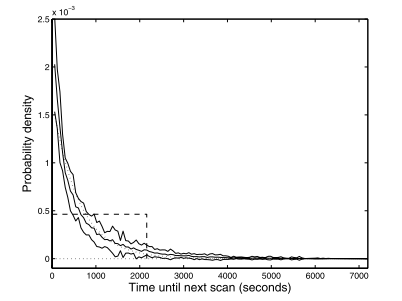
\includegraphics{../images/random_scan_characteristic.png}
\end{figure}

\begin{figure}[!h]
\caption{\label{pheromonechar} Pheromone mobility}
   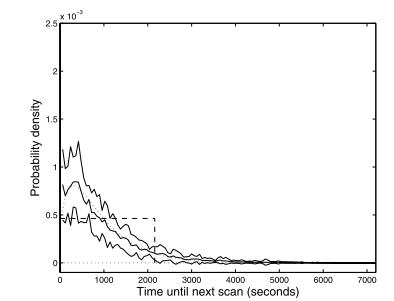
\includegraphics{../images/pheromone_scan_characteristic.png}
\end{figure}

\newpage

\subsection{Never scanned area}

In this tableau below, we can see the results about the percentage of the map never scanned.\\

\begin{tabular}{|c|c|c|c|}
\hline
	      & Max & Median & Min \\
	      \hline
	Random & 16.2\% & 3.2\% & 0.5\% \\
	\hline
	Pheromone & 0.21\% & 0.03\% & 0.01\% \\
	\hline
\end{tabular}\\\\

It represents the maximum, median and minimum uncovered area for the ten runs. These numbers clearly show the ability of the pheromone model to cover the complete area. 

\newpage

\subsection{Connectivity}

\begin{figure}[!h]
\caption{\label{randomconnect} Random. Number of UAVs in contact with C\&C (max, average, min)}
   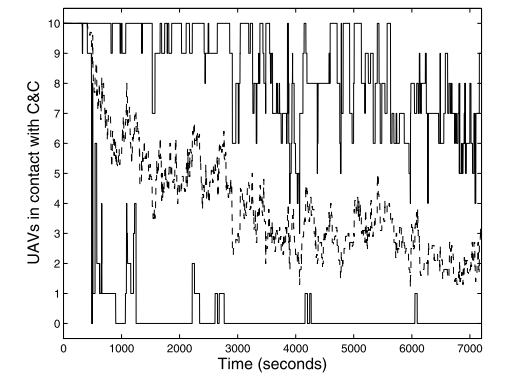
\includegraphics{../images/random_resultat_connectivite.png}
\end{figure}

\newpage

\begin{figure}[!h]
\caption{\label{pheromoneconnect}Pheromone. Number of UAVs in contact with C\&C (max, average, min)}
   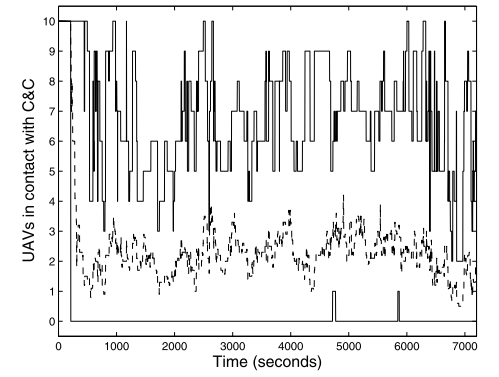
\includegraphics{../images/pheromone_resultat_connectivite.png}
\end{figure}

In Figure \ref{randomconnect} and Figure \ref{pheromoneconnect},we can see the number of UAV wich can communicate with the C\&C.  The  graphs  show the maximum, average, and minimum of this number for the ten runs. We saw that both models don't provide good connectivity. There are not enough UAV to have a fully connected communication graph. Because of the pheromone logic that pushes the UAVs away from each other, this model have low connectivity. Whereas the random model have a high connectivity at the beginning of the run. Then with the random trajectory of each UAV, they move away from each others and finally this model finishes to have the same poor connectivity as the pheromone model.
